\chapter{THỰC NGHIỆM VÀ ĐÁNH GIÁ}

% Generated by python -m scripts.render_report; do not hand edit.

\section{Trạng thái dữ liệu và phạm vi phép đo}

Corpus chính gồm 2.500 bài thuộc 10 lĩnh vực, 250 bài/lĩnh vực. Bộ 20 query có hai query/lĩnh vực. Pool dùng BiMM có 669 cặp, 0 nhãn confirmed; mẫu kiểm tra chéo gồm 134 cặp.

Ba baseline pooling: TF-IDF Cosine sublinear/smoothed/L2; binary presence Cosine không IDF; BM25 với $k_1=1{,}2$, $b=0{,}75$, IDF một lần. Cùng corpus và tokenizer, hợp Top-20; TF-IDF đã đối soát SearchEngine.

\textbf{P@10, Recall@10, F1@10, MAP và NDCG@10: chưa đo chính thức.} Nhãn pending không được biến thành relevance. Bảng theo query/lĩnh vực dưới đây là độ trễ thật, không thay cho chất lượng truy xuất.

\section{Môi trường và thiết lập}

Lần đo UTC: 2026-10-16T13:42:48.188882+00:00. Python 3.13.5; Windows-11-10.0.26300-SP0; CPU AMD64 Family 25 Model 117 Stepping 2, AuthenticAMD; 16 logical CPU.

Mỗi query lặp 100 lần, 5 lượt warm-up trên toàn query set, Top-10. Chỉ mục đã nạp; đo gồm chuẩn hóa, BiMM, lọc và truy xuất, không gồm khởi động Python/nạp từ điển/đĩa hay vẽ giao diện. C4 thuần và fallback C3 được đo độc lập.

\section{Kết quả độ trễ và dung lượng}

\begin{table}[htbp]
\centering
\begin{tabular}{|l|r|r|r|r|}
\hline
Cấu hình & Mean (ms) & P95 (ms) & Rỗng & Số đo \\
\hline
C1 & 0.994 & 1.992 & 0 & 2000 \\
C2 & 0.463 & 1.034 & 0 & 2000 \\
C3 & 0.772 & 1.737 & 0 & 2000 \\
C4 & 0.487 & 1.355 & 200 & 2000 \\
C4 + C3 & 0.503 & 1.226 & 0 & 2000 \\
\hline
\end{tabular}
\caption{Độ trễ trên corpus chính, BiMM thật.}
\end{table}

\begin{table}[htbp]
\centering
\begin{tabular}{|l|r|r|r|l|}
\hline
Cấu hình & Phục vụ (byte) & TDV (byte) & Giảm/C1 & Mục tiêu 30\% \\
\hline
C1 & 9621765 & 0 & 0.00\% & không đạt \\
C2 & 6987156 & 0 & 27.38\% & không đạt \\
C3 & 8748327 & 0 & 9.08\% & không đạt \\
C4 & 6542944 & 1834419 & 32.00\% & đạt \\
C4 + C3 & 15291271 & 1834419 & -58.92\% & không đạt \\
\hline
\end{tabular}
\caption{Dung lượng chỉ mục đơn và gói triển khai fallback.}
\end{table}

C4 thuần trả kết quả rỗng ở Q04, Q15; phép đo C4 + C3 dùng chỉ mục C3 riêng để khôi phục truy vấn, không giữ term đã bị xóa trong chỉ mục C4.

Mục tiêu mean dưới 30 ms: đạt. Tỷ lệ giảm âm có nghĩa dung lượng tăng. Phải giữ C3 nếu triển khai fallback; không sử dụng riêng dung lượng C4 để kết luận cho cả gói. Tốc độ thấp hơn không chứng minh relevance tốt hơn.

\begin{figure}[htbp]\centering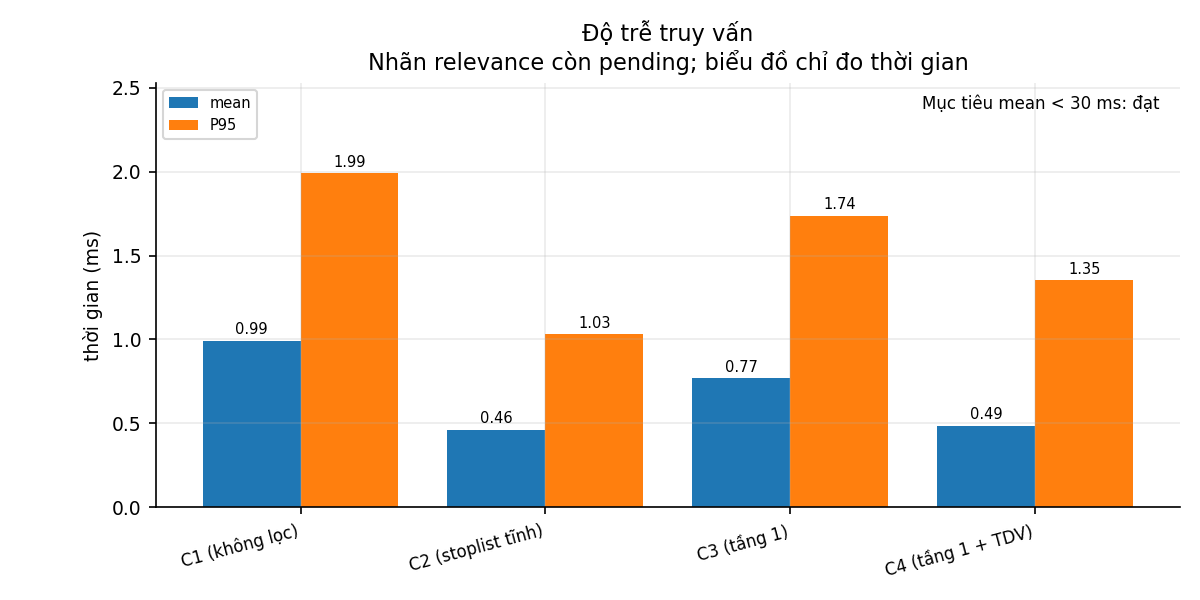
\includegraphics[width=.9\textwidth]{figures/fig_latency.png}\caption{Mean/P95 truy vấn BiMM.}\end{figure}

\begin{figure}[htbp]\centering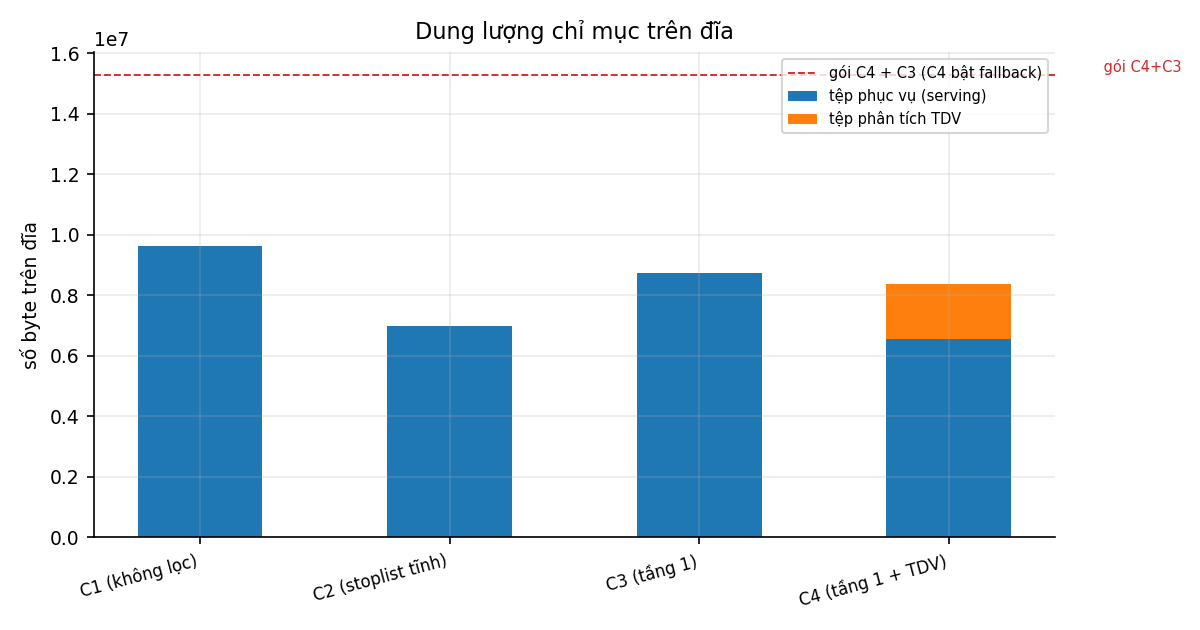
\includegraphics[width=.9\textwidth]{figures/fig_index_size.png}\caption{Dung lượng phục vụ, phân tích và gói fallback.}\end{figure}

\section{Thống kê TDV trên corpus đa lĩnh vực}

Mật độ gốc 0.03731830; chấm 31076 term, 666 điểm âm dưới dung sai. Bảo vệ 77 term theo whitelist/policy hợp từ; lọc thật 589 term. Thời gian TDV 12.641 giây, one-shot trên đủ 2.500 bài. Đây là tiêu chí hình học, không phải nhãn không liên quan ngữ nghĩa.

\begin{figure}[htbp]\centering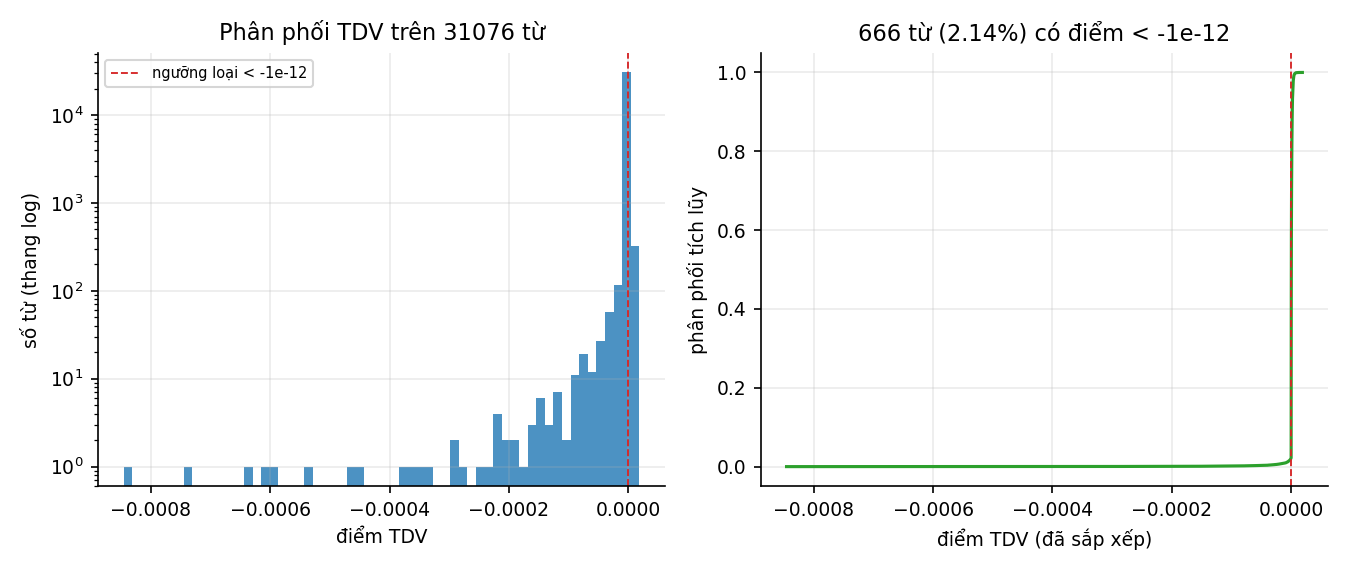
\includegraphics[width=.9\textwidth]{figures/fig_tdv_distribution.png}\caption{Phân bố TDV thực, không ép hình chữ U.}\end{figure}

\clearpage\section{Toàn bộ query và phân tích theo lĩnh vực}

\begin{longtable}{|l|p{.48\textwidth}|r|r|r|r|}
\hline
Query & Nội dung & C1 & C2 & C3 & C4 \\
\hline
\endhead
Q01 & lương tối thiểu & 0.153 & 0.091 & 0.188 & 0.089 \\
Q02 & biển cấm đỗ xe ô tô ở Hà Nội mất hiệu lực thì người dân đỗ xe ở đâu & 1.457 & 0.870 & 1.638 & 0.998 \\
Q03 & có nên tha thứ cho người vợ ngoại tình & 1.043 & 0.275 & 0.765 & 0.401 \\
Q04 & tâm sự gia đình & 0.198 & 0.244 & 0.162 & 0.031 \\
Q05 & nghiên cứu lõi băng để khám phá quy luật biến đổi khí hậu & 0.809 & 0.460 & 0.726 & 0.303 \\
Q06 & Trung Quốc xây trạm không gian và Nga phóng tàu lên ISS khác nhau như thế nào & 1.537 & 0.900 & 1.248 & 0.913 \\
Q07 & cổ phiếu & 0.066 & 0.055 & 0.107 & 0.079 \\
Q08 & lãi suất cơ bản và chính sách tiền tệ của Fed ảnh hưởng thị trường ra sao & 1.348 & 0.500 & 0.798 & 0.479 \\
Q09 & điều tra vụ biển thủ hơn 8,7 tỷ đồng cá độ bóng đá đã được xử lý ra sao & 1.596 & 0.502 & 1.377 & 0.379 \\
Q10 & đường dây chạy án trong vụ PMU18 & 0.833 & 0.289 & 0.362 & 0.238 \\
Q11 & ung thư & 0.064 & 0.087 & 0.074 & 0.102 \\
Q12 & mỡ máu cao nếu không điều trị có thể gây những biến chứng gì & 1.190 & 0.379 & 1.199 & 1.118 \\
Q13 & vì sao Mỹ vẫn chưa tìm thấy vũ khí cấm ở Iraq & 1.055 & 0.527 & 0.901 & 0.563 \\
Q14 & xác nhận danh tính hài cốt lính Mỹ mất tích trong Chiến tranh Triều Tiên & 1.037 & 0.697 & 0.653 & 0.457 \\
Q15 & vô địch & 0.091 & 0.117 & 0.144 & 0.019 \\
Q16 & Việt Nam đăng cai một vòng bảng Tiger Cup 2004 và các trận chung kết diễn ra thế nào & 1.723 & 0.814 & 1.499 & 1.388 \\
Q17 & cảnh nóng và trang phục hở trong phim truyền hình Việt Nam gây tranh luận như thế nào & 1.697 & 0.899 & 1.150 & 1.007 \\
Q18 & ca khúc và chương trình biểu diễn âm nhạc của nghệ sĩ & 1.182 & 0.464 & 0.502 & 0.275 \\
Q19 & virus máy tính đánh cắp mật khẩu Windows và cách phòng tránh & 1.224 & 0.412 & 0.643 & 0.351 \\
Q20 & dịch vụ phần mềm và thông tin di động được doanh nghiệp cung cấp cho khách hàng ra sao & 1.569 & 0.683 & 1.302 & 0.555 \\
\hline
\caption{Mean ms của toàn bộ 20 query.} \\
\end{longtable}

\begin{table}[htbp]
\centering
\begin{tabular}{|l|r|r|r|r|r|}
\hline
Lĩnh vực & Query & C1 & C2 & C3 & C4 \\
\hline
Chính trị – Xã hội & 2 & 0.805 & 0.481 & 0.913 & 0.543 \\
Đời sống & 2 & 0.621 & 0.259 & 0.464 & 0.216 \\
Khoa học & 2 & 1.173 & 0.680 & 0.987 & 0.608 \\
Kinh doanh & 2 & 0.707 & 0.277 & 0.452 & 0.279 \\
Pháp luật & 2 & 1.215 & 0.395 & 0.870 & 0.309 \\
Sức khỏe & 2 & 0.627 & 0.233 & 0.637 & 0.610 \\
Thế giới & 2 & 1.046 & 0.612 & 0.777 & 0.510 \\
Thể thao & 2 & 0.907 & 0.465 & 0.821 & 0.703 \\
Văn hóa & 2 & 1.440 & 0.681 & 0.826 & 0.641 \\
Vi tính & 2 & 1.397 & 0.548 & 0.973 & 0.453 \\
\hline
\end{tabular}
\caption{Mean ms theo 10 lĩnh vực; chỉ hai query/lĩnh vực.}
\end{table}

Mỗi lĩnh vực chỉ có hai query nên kết quả nhóm chưa đủ để suy rộng. Các bảng chất lượng toàn query/nhóm sẽ do evaluator xuất khi qrels đủ điều kiện, không thay dữ liệu thiếu bằng số 0.


\section{Định nghĩa chỉ số chất lượng và điều kiện công bố}

Cả bốn cấu hình dùng cùng corpus, query và qrels. Relevance là nhãn theo nội
dung của từng cặp query--document, không phải cùng lĩnh vực. Grade 0 là không
liên quan, grade 1 là liên quan một phần, grade 2 là đáp ứng trực tiếp;
grade lớn hơn 0 là relevant khi tính các chỉ số nhị phân.

Với $R_q$ là tập relevant đã biết của truy vấn $q$, $L_q^K$ là Top-$K$ kết quả:
\begin{align}
P@K &= \frac{|R_q\cap L_q^K|}{K},\\
Recall@K &= \frac{|R_q\cap L_q^K|}{|R_q|},\\
F1@K &= \frac{2\,P@K\,Recall@K}{P@K+Recall@K}.
\end{align}
Khi mẫu số bằng 0 quy ước kết quả bằng 0. Query không có relevant giữ điểm 0
trong bình quân macro và được đếm riêng; ranking rỗng cũng giữ 0, không loại khỏi
bình quân để làm đẹp kết quả. Mặc định $K=10$ cho Precision/Recall/F1/NDCG.

\begin{equation}
AP(q)=\frac{1}{|R_q|}\sum_{r=1}^{L}P@r\;rel(r),\qquad
MAP=\frac{1}{|Q|}\sum_{q\in Q}AP(q).
\end{equation}
$L$ là toàn ranking có sẵn (độ sâu mặc định bằng số tài liệu trong corpus).
Nếu cố ý cắt ranking phải ghi AP@depth, không gọi là MAP toàn ranking.
Document không có điểm dương không được bịa thành kết quả để đủ độ sâu.

\begin{equation}
DCG@K=\sum_{r=1}^{K}\frac{2^{grade(r)}-1}{\log_2(r+1)},\qquad
NDCG@K=\frac{DCG@K}{IDCG@K}.
\end{equation}
$IDCG$ lấy thứ tự grade lý tưởng từ qrels, không chỉ từ tài liệu đã trả về.
Nếu $IDCG=0$ thì NDCG bằng 0.

Bộ đánh giá chính thức kiểm tra schema, SHA256 corpus thực/manifest, SHA256
query, trạng thái nhãn, assessor và metadata preprocessing. Pending không được
tự diễn giải thành nhãn đã xác nhận. Khi chưa sẵn sàng, kết quả ghi
\texttt{unmeasured} và không xuất bảng điểm 0 như một phép đo chất lượng.
Các bảng theo query và 10 lĩnh vực được evaluator xuất khi qrels đủ điều kiện.

\section{Kiểm định tách từ và cấu trúc tra cứu}

Tập chuẩn bị cho M1 gồm 150 câu có nguồn từ corpus chính, 15 câu/lĩnh vực,
được lưu ở \texttt{data/gold/}. Gợi ý FMM/BMM/BiMM chỉ phục vụ gán nhãn;
không gọi output của thuật toán là gold. Người gán cần xác nhận phân đoạn,
assessor, nội dung chuẩn hóa và hash trước khi đo.

Đánh giá dùng khớp span từ trên cùng chuỗi âm tiết chuẩn hóa: một từ chỉ đúng
khi cả đầu và cuối span đều khớp. Precision là số span khớp chia span dự đoán,
Recall chia span gold, F1 là trung bình điều hòa. Không dùng tỷ lệ khớp ký tự
thay cho độ chính xác phân đoạn từ. Quy trình nhập nhãn phải từ chối phân đoạn
làm mất/thêm/đổi thứ tự âm tiết. Tệp hiện có 150/150 câu mang cờ xác nhận;
đường đánh giá chỉ được dùng làm kết luận sau khi nhãn gold được duyệt nội dung.
Rà soát bản gold hiện tại thấy 102 câu giữ nguyên toàn bộ gợi ý BiMM. Ít nhất
SG010, SG053 và SG089 có phân đoạn cần người gán xem lại; ví dụ SG010 ghép
``độc\_đáo\_để''. Sự trùng gợi ý không tự chứng minh nhãn sai,
nhưng số đo trên nhãn hiện có cần được kiểm tra độc lập trước khi coi là kết luận
cuối. Bảng F1 dưới đây được sinh lại từ kết quả đánh giá khớp bản gold đang dùng;
nếu thiếu hoặc lệch bản gold thì không được giữ số cũ.
\IfFileExists{segmentation_results.tex}{% Generated by python -m scripts.render_report; do not hand edit.

\textbf{Phân đoạn từ: số đo trên nhãn hiện có, tạm thời khi audit gold còn mở.} Word-span micro trên 150 câu; chỉ công bố là kết quả cuối sau khi duyệt các cặp nghi vấn.

\begin{table}[htbp]
\centering
\begin{tabular}{|l|r|r|r|}
\hline
Thuật toán & Precision & Recall & F1 \\
\hline
FMM & 0.9517 & 0.9643 & 0.9580 \\
BMM & 0.9561 & 0.9688 & 0.9624 \\
BiMM & 0.9561 & 0.9688 & 0.9624 \\
\hline
\end{tabular}
\caption{Word-span micro trên 150 câu gold hiện có; cần rà soát nhãn.}
\end{table}
}{\par\emph{Chưa có bảng F1 tách từ hợp lệ cho bản gold hiện tại.}}

Đối chứng Trie và Set phải dùng cùng từ điển, câu, cửa sổ và luật BiMM. Kiểm tra
output parity trước khi so tốc độ. Thời gian khởi tạo và bộ nhớ Python qua
\texttt{tracemalloc} tách khỏi thời gian tách câu; không gọi đây là toàn bộ RAM
tiến trình. Không mặc định Trie luôn nhanh hơn hash set.
Phép đo thật trên 150 câu mẫu và 100 bài đầu của corpus khóa (10 vòng lặp,
2 lượt warm-up) có 750 đối soát FMM/BMM/BiMM, không có token nào lệch.
Trên mẫu câu, mean FMM là 0,2328~ms (Trie) so với 0,1147~ms (Set), BiMM là
0,4557 so với 0,1958~ms; trên lát cắt corpus, BiMM là 6,5355 so với
2,6611~ms/bài. Như vậy bản Trie \emph{hiện tại} chậm hơn Set khoảng 2--2,5
lần trong hai workload này. Nguyên nhân triển khai là mỗi độ dài ứng viên lại
tra từ gốc Trie thay vì dùng một lượt dò tiền tố; đây không phải kết luận rằng
Trie nói chung chậm hơn. Đỉnh heap Python khi dựng Trie/Set lần lượt là
20.985.701/15.368.109 byte, không phải RSS. Chi tiết và dữ liệu gốc nằm trong
\texttt{results/lookup/trie\_vs\_set.json} và tài liệu benchmark kèm repo.

\section{Kiểm chứng triển khai}

\subsection{TF-IDF, Cosine và persistence}

Kiểm thử toán học dùng fixture tính tay và đối soát scikit-learn với cùng
analyzer/sublinear TF/smoothed IDF/L2, gồm từ lặp và token một ký tự.
Kiểm tra query rỗng, OOV, vector 0, stopword, hòa điểm, query dùng IDF corpus.
Kiểm thử save/load kiểm tra SHA256 artifact, source và tài nguyên; từ chối
tokenizer không thể kiểm chứng và nguồn bị thay đổi.

\texttt{explain()} phân rã bằng tích trọng số query/document đã L2; tổng phải
bằng điểm Cosine trong sai số số thực. Audit đầu-cuối đối chiếu từng kết quả
Top-10 của cả 20 query ở bốn cấu hình và kiểm tra nội dung pool với corpus khóa.

\subsection{TDV}

Đường tham chiếu độc lập dựng ma trận Cosine trực tiếp sau khi xóa từng chiều,
chuẩn hóa lại rồi tính mật độ. Đường nhanh dùng cấu trúc thưa và cập nhật tổng
vector chính xác. Kiểm thử gồm zero vector, một tài liệu, term xuất hiện mọi
tài liệu, dữ liệu ngẫu nhiên, và phản ví dụ cho cách xóa chiều mà không L2 lại.
Không sao chép kết quả tham chiếu làm output của đường tối ưu.

\subsection{Maximum Matching và giao diện}

FMM/BMM/BiMM được kiểm tra bằng từ điển fixture minh bạch, thứ tự trọng tài,
OOV xen kẽ từ đã biết và ranh giới dấu câu. Lead còn dùng oracle Set trực tiếp
độc lập trên từ điển/câu ngẫu nhiên; trace phải tái dựng đúng output khi sắp
terminal action theo vị trí, trong khi thứ tự bước BMM vẫn phản ánh quét lùi.
AppTest chạy mã Streamlit thật cho trang chủ, ba phương pháp, tầng 1, tìm kiếm,
explain, OOV và Analytics.

Báo cáo kiểm chứng đầy đủ và số test cuối nằm ở
\texttt{docs/integration\_status.md}; audit JSON ghi hash, số bài và sai số
phân rã Cosine. Fixture không được đưa vào bảng kết quả corpus chính.

\section{Giới hạn và kết luận}

Đường đánh giá đã tính chất lượng trên 669/669 cặp có cờ xác nhận. Các giá trị
MAP, P@10 và NDCG@10 trong bảng đầu chương là số đo trên tệp nhãn lúc chạy;
không diễn giải thứ hạng giữa các cấu hình là ưu thế có ý nghĩa thống kê hoặc
suy rộng sang kho ngữ liệu khác. Hai phiếu rà soát bằng AI đã liệt kê 37 cặp
qrels không trùng nhau; Team7 gửi quyết định cho cả 37 và sau đó sửa riêng
Q16/\texttt{vn\_f4f2b5ae9443c172} từ mức 2 xuống mức 1. Phép đo trong bảng
đã chạy lại trên qrels mới (SHA256 bắt đầu \texttt{697fafc7}); không dùng
CSV trước lần nhập. Nguồn chấm độc lập M1 vẫn chưa được xác minh, nên kết luận
ngữ nghĩa còn tạm thời dù cổng kỹ thuật đánh giá đã cho phép. Chi tiết nằm
trong biên bản \path{results/label_review_resolution.json}.
Tập query nhỏ (hai/lĩnh vực) và qrels pooling có thiên lệch theo các hệ thống
đóng góp; tài liệu relevant bị cả ba baseline bỏ sót không có nhãn, không có
hướng sai lệch cố định của MAP/Recall so với relevance đầy đủ.

Maximum Matching phụ thuộc từ điển, dễ nhập nhằng với tên riêng, từ mới và cụm
dài; từ điển rộng có cả thành ngữ không đồng nghĩa là phân đoạn tốt. Chính sách
chuẩn hóa bỏ số/URL/email và giữ chữ Latin vay mượn cần được cân nhắc khi đọc
query chuyên ngành. Bag-of-words giữ phủ định không có nghĩa đã suy luận đúng
ngữ nghĩa phủ định.

Số đo latency là warm process trên một máy, không phải cam kết độ trễ mọi máy
hay mọi kích thước corpus. Kết quả kích thước phải tách chỉ mục C4 thuần khỏi gói
C4+C3. Phần triển khai, tích hợp và phép tính đã chạy; kết luận chất lượng cuối
cần được cập nhật sau khi mẫu kiểm tra chéo và gold tách từ được duyệt.
